%% LaTeX-Beamer template for KIT design
%% by Erik Burger, Christian Hammer
%% title picture by Klaus Krogmann
%%
%% version 2.1
%%
%% mostly compatible to KIT corporate design v2.0
%% http://intranet.kit.edu/gestaltungsrichtlinien.php
%%
%% Problems, bugs and comments to
%% burger@kit.edu

\documentclass[18pt]{beamer}
\usepackage[utf8]{inputenc}
%% SLIDE FORMAT

% use 'beamerthemekit' for standard 4:3 ratio
% for widescreen slides (16:9), use 'beamerthemekitwide'

\usepackage{templates/beamerthemekit}
% \usepackage{templates/beamerthemekitwide}

%% TITLE PICTURE

% if a custom picture is to be used on the title page, copy it into the 'logos'
% directory, in the line below, replace 'mypicture' with the 
% filename (without extension) and uncomment the following line
% (picture proportions: 63 : 20 for standard, 169 : 40 for wide
% *.eps format if you use latex+dvips+ps2pdf, 
% *.jpg/*.png/*.pdf if you use pdflatex)

\titleimage{banner}

%% TITLE LOGO

% for a custom logo on the front page, copy your file into the 'logos'
% directory, insert the filename in the line below and uncomment it

\titlelogo{logo}

% (*.eps format if you use latex+dvips+ps2pdf,
% *.jpg/*.png/*.pdf if you use pdflatex)

%% TikZ INTEGRATION

% use these packages for PCM symbols and UML classes
% \usepackage{templates/tikzkit}
% \usepackage{templates/tikzuml}

% the presentation starts here

\title[Vortrag Geometrie I]{Geometrie I}
\subtitle{Problemstellungen in 0 bis 3 Dimensionen}
\author{Lukas Böhm, Eric Sallermann, Vincent Schüßler}

\institute{ICPC Basispraktikum SS2014}

\beamertemplatenavigationsymbolsempty

\begin{document}

% change the following line to "ngerman" for German style date and logos
\selectlanguage{ngerman}

%title page
\begin{frame}
\titlepage
\end{frame}

%table of contents
\begin{frame}{Übersicht}
\tableofcontents
\end{frame}

\begin{frame}{Floating Point Beispiel}
	\lstset{
		language=C++,
		tabsize=2
	}
	\lstinputlisting{error.cpp}
	Ausgabe?
\end{frame}

\begin{frame}{Unerwartete Ergebnisse}
	\begin{exampleblock}{Ausgabe}
		3.5999999046325683594 \\
		false\\
		false
	\end{exampleblock}
	3.6 nicht darstellbar \\
	Rundungsfehler \\
	Seltsame Sonderwerte:
	\begin{itemize}
		\item NaN
		\item Inf
		\item +-0
	\end{itemize}
\end{frame}

\begin{frame}{IEEE 754 Knigge}
	\begin{itemize}
		\item Floats \& Doubles möglichst vermeiden
		\item Wenn nötig, erst ganz spät von Ganzzahl zu Fließkomma wechseln
		\item Bitte KEIN float und NUR double benutzen
		\item Keine direkten Vergleiche
	\end{itemize}
\end{frame}

\begin{frame}{Punkte}
	\begin{block}{Rotation um Ursprung (2D)}
		$
		\begin{bmatrix}
			x'\\
			y'
		\end{bmatrix}
		=
		\begin{bmatrix}
			\cos(\theta) & -\sin(\theta)\\
			\sin(\theta) & \cos(\theta)
		\end{bmatrix}
		\times
		\begin{bmatrix}
			x\\
			y
		\end{bmatrix}
		$
	\end{block}
	\begin{itemize}
		\item Rotationen um Punkte mittels Translationen
		\item In 3D um Achsen $\Rightarrow$ Zusätzliche Identitätszeile
	\end{itemize}
	
	Schreibt man sich einmal auf und sucht es sich bei Gelegenheit wieder raus
\end{frame}

\begin{frame}{Geraden}
	\begin{block}{Darstellung}
		Darstellung mittels 3 Komponenten $a$, $b$, $c$:
		\begin{center}
			$ax + by + c = 0$
		\end{center}
	\end{block}
	\begin{itemize}
		\item Ermöglicht Spezialfall vertikale Linie
		\item Normalisierung mit $b = 0$ (vertikal) oder $b = 1$ (sonst) vereinfacht Vergleiche
	\end{itemize}
\end{frame}

\begin{frame}{Trigonometrie}
	\begin{columns}
	\column{.6\textwidth}
	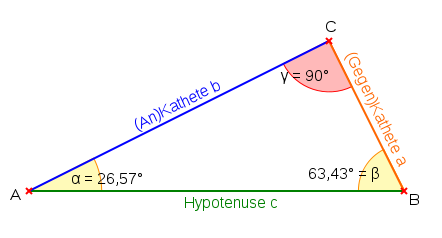
\includegraphics[width=1.1\textwidth,height=.8\textheight,keepaspectratio]{dreieck.png}
	\column{.4\textwidth}
	\begin{itemize}
		\item $\sin \alpha = \frac{Gegenkathete}{Hypotenuse}$
		\item $\cos \alpha = \frac{Ankathete}{Hypotenuse}$
		\item $\tan \alpha = \frac{Gegenkathete}{Ankathete}$
	\end{itemize}
	\end{columns}
	Quelle: \url{http://upload.wikimedia.org/wikipedia/commons/5/56/RechtwinkligesDreieck.svg}
\end{frame}

\begin{frame}{Trigonometrie}
	\begin{center}
		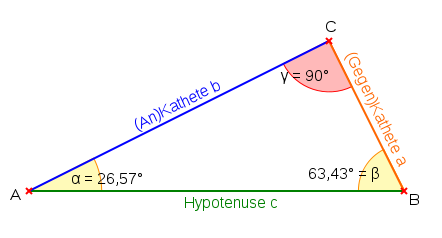
\includegraphics[width=0.6\textwidth,height=.8\textheight,keepaspectratio]{dreieck.png}
	\end{center}
	
	\begin{block}{Cosinusregel}
		\begin{itemize}
			\item $c^2 = a^2 + b^2 - 2 * a * b * \cos \gamma$
			\item $b^2 = a^2 + c^2 - 2 * a * c * \cos \beta$
			\item $a^2 = b^2 + c^2 - 2 * b * c * \cos \alpha$
		\end{itemize}
	\end{block}
\end{frame}

\begin{frame}{Trigonometrie}
	\begin{center}
		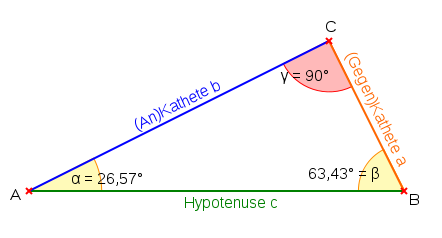
\includegraphics[width=0.6\textwidth,height=.8\textheight,keepaspectratio]{dreieck.png}
	\end{center}
	
	\begin{block}{Sinusregel}
		$\frac{a}{\sin \alpha} = \frac{b}{\sin \beta} = \frac{c}{\sin \gamma} = \frac{a * b * c}{2 * F}$,
		wobei F der Flächeninhalt des Dreiecks ist.
	\end{block}
\end{frame}

\begin{frame}{Trigonometrie}
	\begin{block}{atan2(y, x)}
		\textit{Gegeben:} Punkt $(x,y)$\\ \ \\
		
		\hangindent+20pt \hangafter=1
		\textit{Rückgabewert:} Winkel (in RAD) zwischen der x-Achse und dem Punkt $(x,y)$. Der Wert hat ein \textbf{positives} Vorzeichen, wenn die Drehung \textbf{gegen} den Uhrzeigersinn erfolgt, ansonsten negatives Vorzeichen.\\ \ \\

		Der Wertebereich ist $-\pi < atan2(y, x) \leq \pi$.
	\end{block}
	
	Hinweis: Um von RAD zu DEG zu konvertieren, ist eine Multiplikation mit $\frac{180}{\pi}$ nötig.
\end{frame}

\begin{frame}{Trigonometrie}
	\begin{block}{Winkelberechnung zwischen drei Punkten}
		\textit{Gegeben:} Drei Punkte $a, o, b$\\
		\textit{Gesucht:} $\sphericalangle aob$\\ \ \\

		Formel: $\cos \phi = \left|\frac{\overrightarrow{oa} \cdot \overrightarrow{ob}}{\norm{\overrightarrow{oa}}_2 * \norm{\overrightarrow{ob}}_2}\right|$\\
	\end{block}
	
	\lstset{
		language=C++,
		tabsize=1
	}
	\lstinputlisting[firstline=52, lastline=59]{vectors.cpp}
\end{frame}


\begin{frame}{Vektoren}
	\begin{itemize}
		\item Definiert durch zwei Punkte und eine Richtung
		\item Skalieren, Verschieben
		\item Länge von Vektoren
		\item (oberes durch Bilder veranschaulicht)
		\item (Code für obiges zum Nachschlagen)
	\end{itemize}
\end{frame}

\begin{frame}{Skalarprodukt, Kreuzprodukt}
	\begin{itemize}
		\item Bedeutung/Aussage von Skalarprodukt und Kreuzprodukt
		\item (Bilder)
		\item (Code)
	\end{itemize}
\end{frame}

\begin{frame}{Winkel zwischen zwei zusammenhängenden Strecken, CCW/Linksknick-Test}
	\begin{itemize}
		\item Winkelberechnung
		\item CCW-Test mit Hilfe des Kreuzprodukts (0 = kollinear, negativ = Rechtsknick, positiv = Linksknick)
		\item (Bilder, toll wa?)
		\item (Code)
	\end{itemize}
\end{frame}

\begin{frame}{Dreiecke/Trigonometrie}
	\begin{itemize}
		\item Wiederholung zu Sinus, Cosinus, Tangens (vielleicht vor Winkelberechnung?)
		\item Cosinus-Regel 
		\item Sinus-Regel
	\end{itemize}
\end{frame}
\begin{frame}{Polygone}
	\begin{columns}
	\column{.55\textwidth}
	\begin{itemize}
		\item \textbf{Polygon}: Fläche begrenzt durch geschlossenen Pfad von Kanten
		\item Darstellung als Folge von Eckpunkten (\texttt{vector<point>}), erster gleich letztem Punkt (also $\langle P_0, P_1, \ldots, P_{n-1}, P_0\rangle$)
		\item \emph{Konvexes} Polygon: Strecke zwischen zwei beliebigen Punkten im Polygon schneidet keine Kante
		\item sonst ist das Polygon \emph{konkav}
	\end{itemize}
	\column{.45\textwidth}
	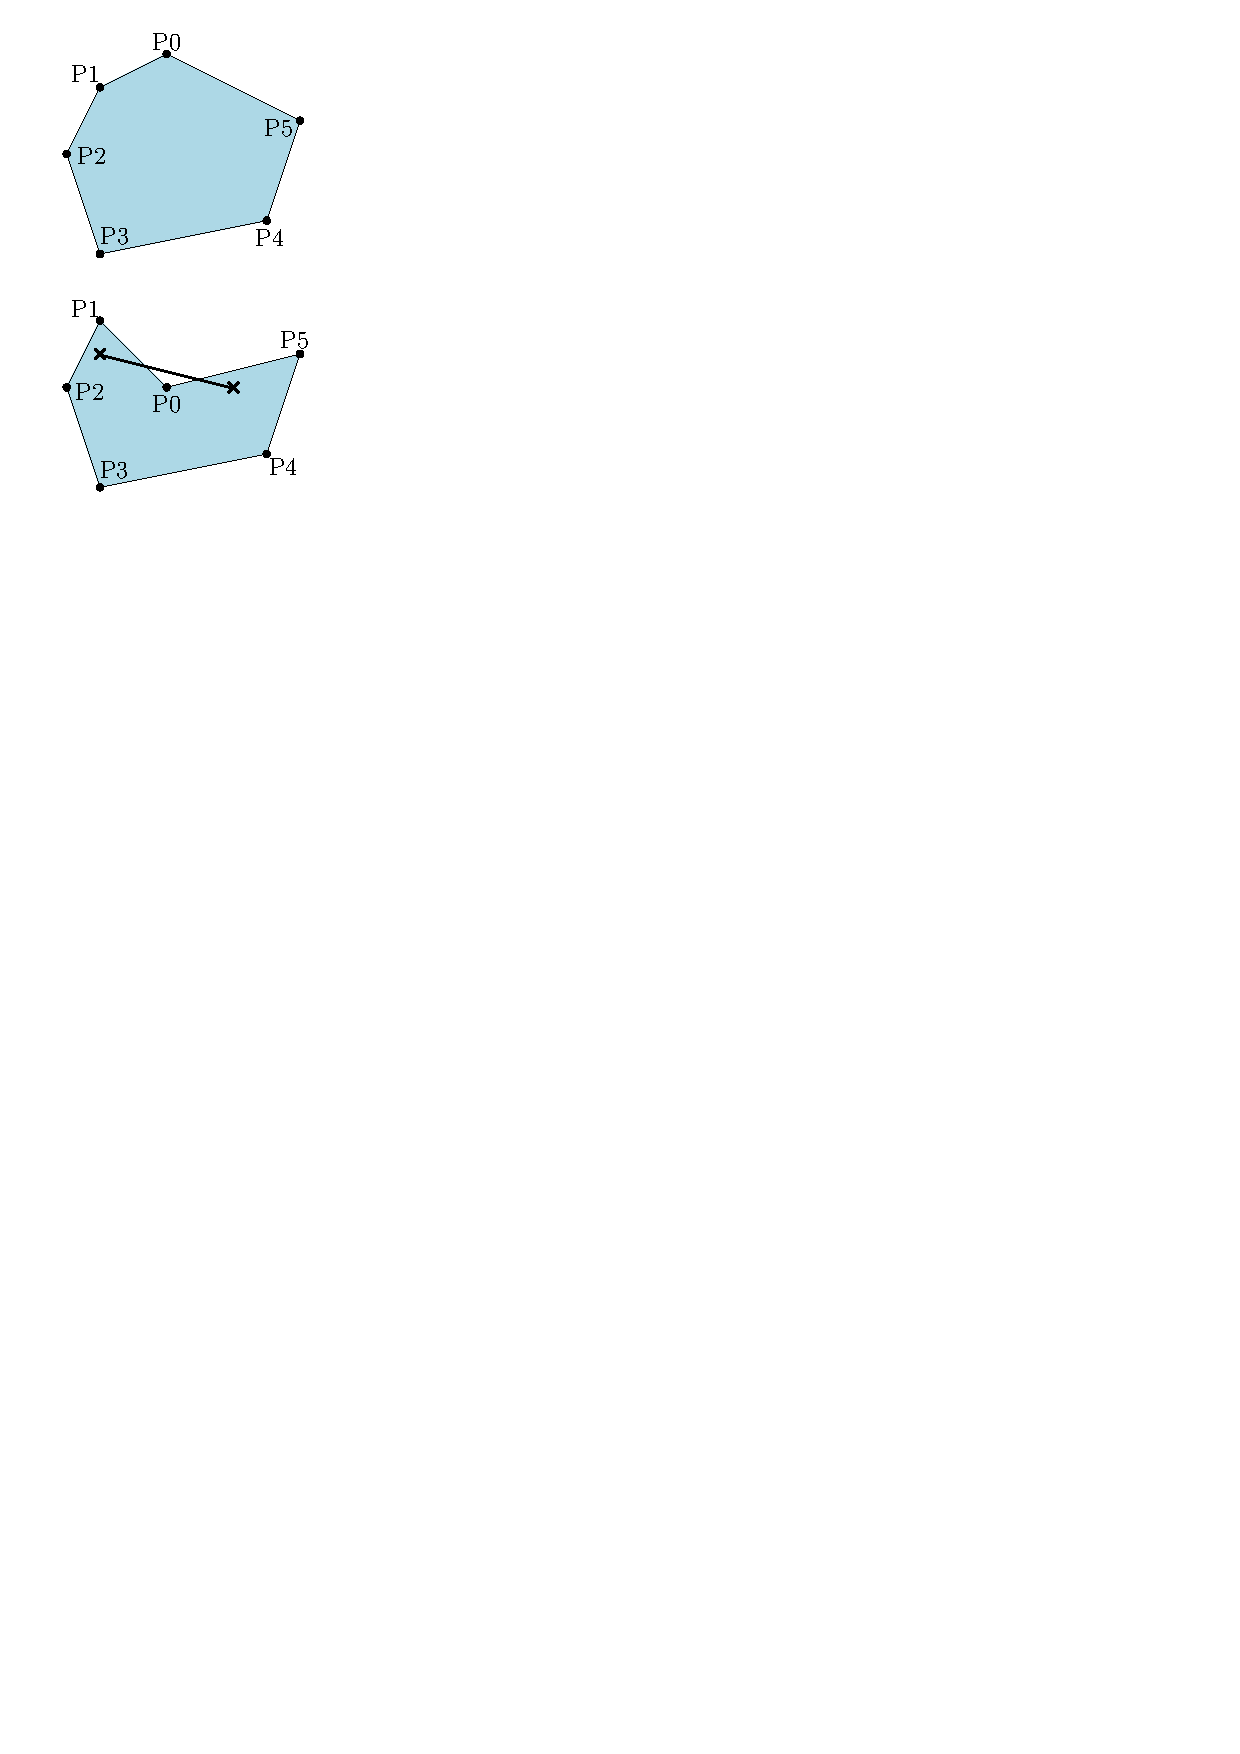
\includegraphics[height=.8\textheight,keepaspectratio]{polygon.pdf}
	\end{columns}
\end{frame}

\begin{frame}{Flächeninhalt}
	\textbf{Problem}: Wie groß ist der Flächeninhalt eines gegebenen Polygons?

	\pause

	\begin{block}{Flächeninhalt}
		\begin{align*}
			A &= \sum_{i=0}^{n-1} \frac{1}{2} (P_i \times P_{i+1})\qquad \textit{($P_n = P_0$)} \\
			  &= \frac{1}{2} ( x_0 y_1 + x_1 y_2 + \ldots + x_{n-1} y_0 - x_1 y_0 - x_2 y_1 - \ldots - x_0 y_{n-1})
		\end{align*}
	\end{block}

	\begin{center}
		
\includegraphics[keepaspectratio,height=3cm]{polygon_area.pdf}
	\end{center}
\end{frame}

\begin{frame}{Überprüfung von Konvexität}
	\textbf{Problem}: Ist ein gegebenes Polygon konvex?
	\begin{itemize}
		\item Sind die Eckpunkte gegen den Uhrzeigersinn aufgelistet, darf es nur Linksknicke geben
		\item $\Rightarrow$ CCW für alle Eckpunkte mit Nachbarn
	\end{itemize}

	\begin{center}
		
\includegraphics[keepaspectratio,height=4cm]{polygon_concave.pdf}
	\end{center}
\end{frame}

\begin{frame}{Konvexität: Implementierung}
	\begin{exampleblock}{Code}
		\lstset{
			language=C++,
			tabsize=2
		}
		\lstinputlisting{convex.cpp}
	\end{exampleblock}
\end{frame}

\begin{frame}{Punkt in Polygon}
	\textbf{Problem}: Liegt ein Punkt in einem gegebenen Polygon?
	\begin{itemize}
		\item Idee: Kanten spannen für Punkte innerhalb des Polygons einen vollen Kreis ($360^\circ,\ 2\pi$) auf
		\item $\Rightarrow$ Winkel zwischen benachbarten Eckpunkten und gegebenem Punkt aufsummieren und mit $2\pi$ vergleichen
	\end{itemize}
	\begin{alertblock}{Achtung}
		Winkel von abgewandten Kanten müssen abgezogen werden! $\Rightarrow$ CCW-Test
	\end{alertblock}
\end{frame}

\begin{frame}{Punkt in Polygon: Beispiele}
\end{frame}

\begin{frame}{Punkt in Polygon: Implementierung}
	\begin{exampleblock}{Code}
		\lstset{
			language=C++,
			tabsize=2
		}
		\lstinputlisting{inside.cpp}
	\end{exampleblock}
\end{frame}


\end{document}
